\chapter{Implementação}
\label{sec-implementacao}

Após a definição do escopo \ref{sec:escopo}, dos requisitos \ref{sec:requisitos-do-jogo}, do diagrama de classes \ref{sec:diagrama-de-classes}, da ideia do jogo \ref{sec:jogo}, do ferramental teórico e prático que será utilizado no desenvolvimento do trabalho \ref{sec-referencial} e uma motivação bem definida, temos uma base sólida para a implementação. Neste capítulo são apresentados os detalhes relacionados à arquitetura do programa implementação do software desenvolvido, bem como algumas das decisões de implementação tomadas com base na seção anterior. O objetivo deste capítulo é fornecer uma visão clara e detalhada de como o software foi estruturado e construído, demonstrando as escolhas técnicas realizadas para atender aos requisitos definidos previamente.

Antes de começar um jogo em \textit{pixel art}, é importante definir o tamanho de cada \textit{tile}; os tamanhos mais comuns são (16 x 16), (32 x 32) e (64 x 64). Para esse trabalho, foi optado o tamanho (64 x 64). É importante que todos os tiles presentes no jogo respeitem o mesmo tamanho para uma melhor harmonia visual, e proporções de objetos compatíveis.

\section{Arquitetura do Jogo}
\label{sec:arquitetura-do-jogo}
O desenvolvimento de um jogo envolve a integração de diversas camadas tecnológicas que, se não bem estruturadas, podem inviabilizar o software futuramente. Pensando em melhorar a estruturação do programa, foi projetado sua arquitetura em alto nível para melhor compreensão do código e seus componentes. A Figura \ref{fig:game-architecture} representa uma visão estática da implementação. O retângulo maior representa o jogo e dentro dele a sua lógica. A parte superior são os recursos que o jogo provê internamente, e a parte inferior são os recursos externos que são utilizados pelo jogo.

\begin{figure}[h!]
    \centering
    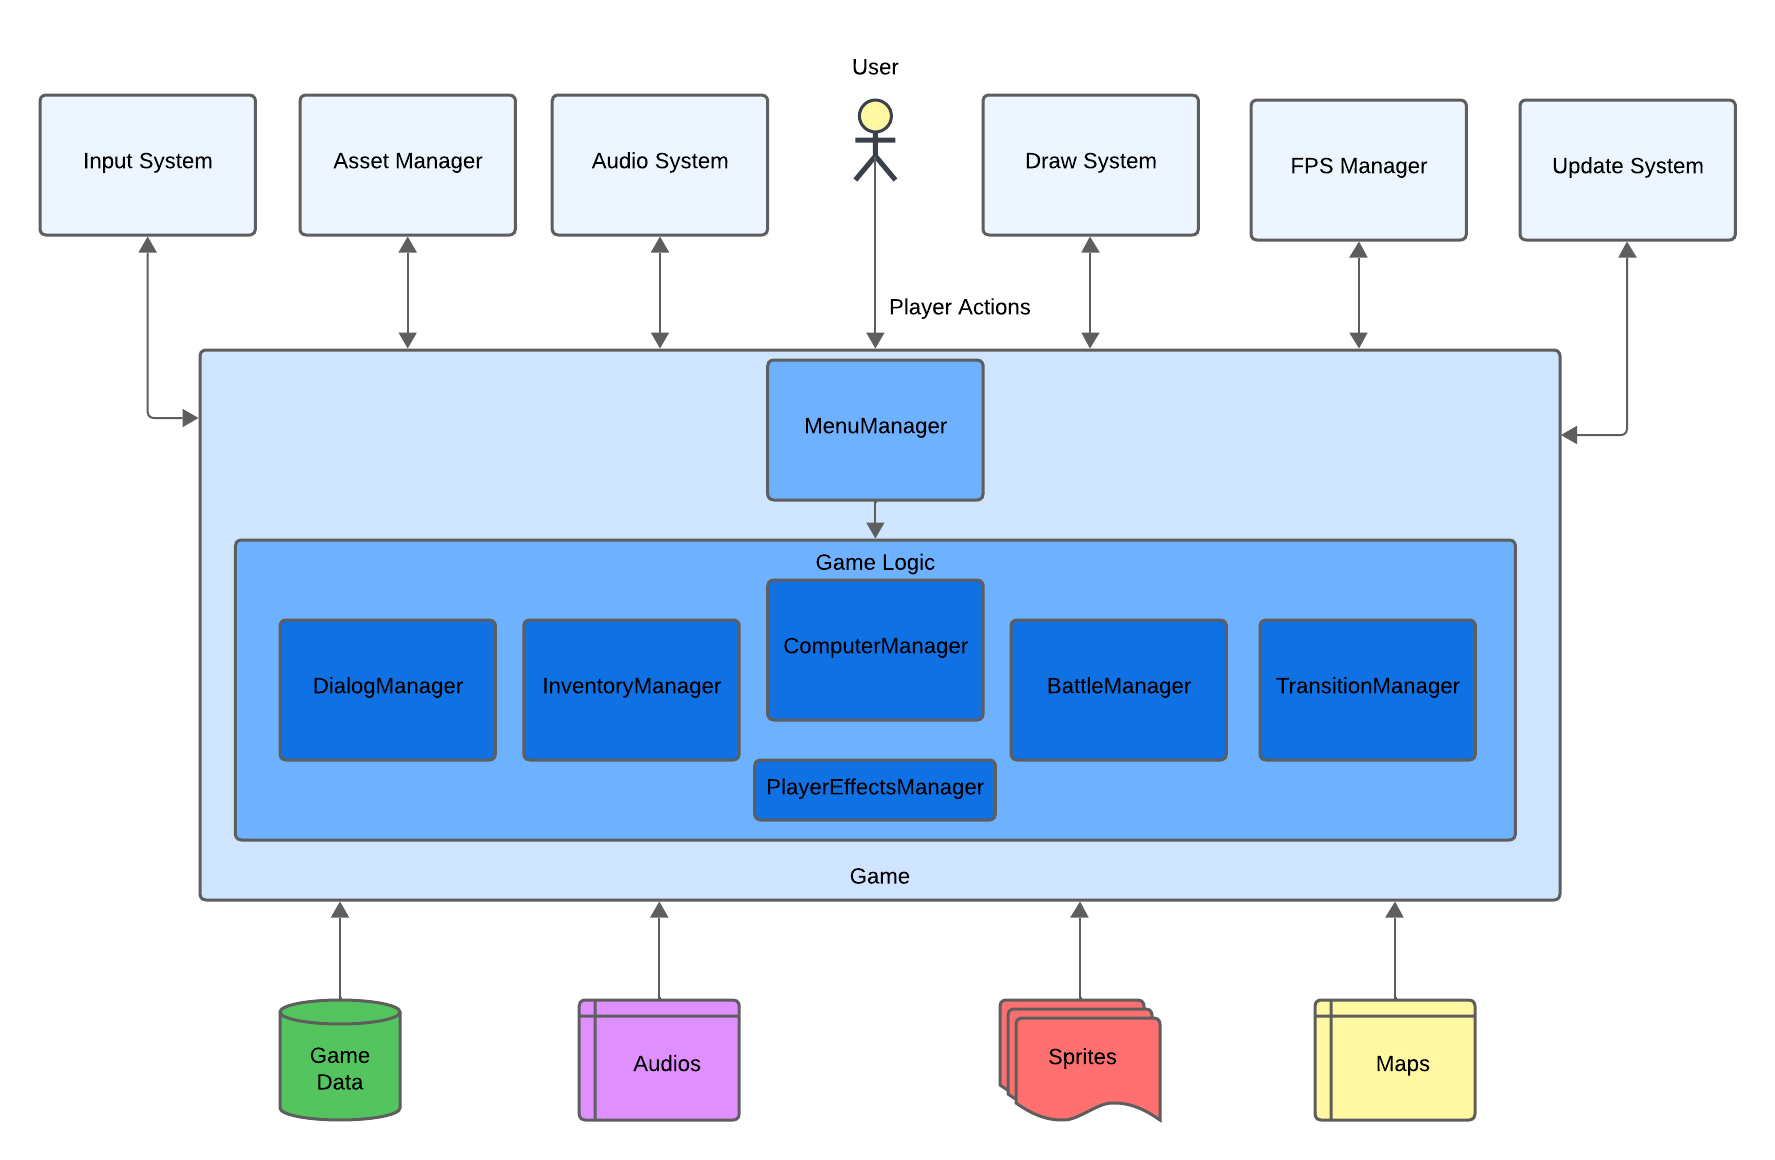
\includegraphics[width=1\linewidth]{figuras/game-architecture.png}
    \caption{Arquitetura do Super LabES World em alto nível}
    \label{fig:game-architecture}
\end{figure}
  

\clearpage
\section{Game Loop do Super Labes World}
\label{sec:game-loop-super-labes-world}
% game loop

O \textit{Game Loop} é o núcleo do jogo e é responsável por manter o jogo em execução contínua até que o jogador feche o programa ou o jogo termine. Nele são continuamente processadas tarefas predefinidas no código do jogo, como ilustrado na listagem \ref{lst-game-loop}.

\lstinputlisting[label=lst-game-loop, caption=Main, language=Python, float=htpb]{codigos/game_loop.py}

A função ilustrada na listagem \ref{lst-game-loop} implementa o \textit{Game Loop} do Super LabES World, composto pelos seguintes passos:
\begin{enumerate}
    \item Preencher o \textit{background} de preto e a área do mapa que não contém tiles também é preenchida com preto (linha 6);
    \item Atualizar o valor do \textit{delta time} (linha 7). Sua importância foi explicada na seção \ref{sec:delta-time};
    \item Verificar o evento de fechar o jogo (linhas 8 a 11);
    \item Chamar a função de \textit{input} que lida com a entrada de controles do jogador (linha 14);
    \item Verificar se o jogador colidiu com um \textit{sprite} de transição (linha 15). Se for o caso então é chamada a função \textit{setup} com os devidos parâmetros do mapa a ser transicionado;
    \item Verificar se o jogador colidiu com alguma caixa de diálogo (linha 16). Se sim então é chamado a função para criar o diálogo com a mensagem;
    \item Atualizar a posição de todos os \textit{sprites} da tela (linha 17). Essa função chama o método \textit{update} de todos os \textit{sprites} contidos no \textit{Group all\_sprites}; 
    \item Desenhar todos os \textit{sprites} da tela;
    \item Verificar se tem alguma sobreposição do jogo. Existem cinco possíveis sobreposições da tela no jogo, são elas;
        \begin{itemize}
        \item \textit{\textbf{dialog\_open: }} Verdadeiro quando o jogador aperta \textit{spacebar} próximo a uma personagem do jogo, então troca de contexto do \textit{loop} principal para o \textit{loop} da classe \textit{Dialog};
        \item \textit{\textbf{inventory\_open: }}Verdadeiro caso o jogador aperte a tecla ''i'', troca o contexto do \textit{loop} principal para o \textit{loop} da classe \textit{Inventory}; 
        \item \textit{\textbf{computer\_open: }} Verdadeiro quando o jogador aperta \textit{spacebar} próximo a \textit{InteractiveObject} com o \textit{item\_id} = \textit{computer}. Então troca de contexto do \textit{loop} principal para o \textit{loop} da classe \textit{Computer};
        \item \textit{\textbf{battle\_open: }}  Verdadeiro quando o jogador responde sim para um desafio de um personagem. Nesse caso troca-se de contexto para a batalha;
        \item \textit{\textbf{choose\_dialog\_open: }} Verdadeiro ao fim de um diálogo de um personagem que contém questões e que não foi derrotado;
    \end{itemize}
\end{enumerate}


% input
A função \textit{input}, ilustrada na listagem \ref{lst-input}, é a responsável por detectar e lidar com todas as entradas de comandos do jogador (exceto a movimentação que será detalhada na seção \ref{sec:personagens}). 
% Nela são definidas todos os possíveis comandos e controles do jogo.
O primeiro passo que deve ser realizado é verificar se o jogador não está bloqueado. Os bloqueios possíveis do jogo são as sobreposições de tela (batalha, inventário, computador) ou se o jogador está dialogando.  
% Por isso antes de verificar a entrada do jogador é conferido os valores das variáveis \textit{booleanas} \textit{dialog\_open} que se verdadeira o jogador está dialogando, \textit{choose\_dialog\_open} se verdadeiro o jogador está na interface de seleção da resposta e \textit{battle\_open} verdadeira quando o jogador está em uma batalha.
Se o jogador não está bloqueado, então é feita a captura da entrada. Os possíveis controles do jogo são:
\begin{itemize}
    \item \textbf{Tecla I: }Abre o inventário e coloca o player no estado bloqueado;
    \item \textbf{Tecla ESC: }Fecha as interfaces de inventário, computador e tira o jogador do estado bloqueado;
    \item \textbf{Tecla \textit{Spacebar}: }A tecla de interação do jogador, quando pressionada é verificado se o jogador está perto a um personagem, ou a um objeto interativo. Quando for o caso a função leva para o respectivo tratamento;
\end{itemize}

\lstinputlisting[label=lst-input, caption=Input, language=Python, float=htpb]{codigos/input.py} 

\section{Principais Funções}
\label{sec:principais-funcoes}
Nessa seção serão detalhadas as principais funções que garantem o funcionamento adequado do jogo desenvolvido. Serão apresentados os módulos centrais, abordando suas finalidades, interações e relevância para o cumprimento dos objetivos do sistema. Além disso, serão discutidas as escolhas realizadas durante o desenvolvimento, evidenciando como essas funções se complementam.

A primeira coisa a se fazer em um projeto Pygame é inicializá-lo invocando o método \textit{pygame.init()}. Isso inicializará todos os módulos do Pygame e permitirá chamadas de funções. Ao executar o programa, a primeira tela que aparece ao jogador é a \textit{home}; essa tela pode levar a quatro outras possíveis transições, sendo elas:
\begin{enumerate}
    \item \textbf{\textit{New: }} Começa um novo jogo;
    \item \textbf{\textit{Credits: }} Abre a tela de créditos;
    \item \textbf{\textit{Controls: }} Abre a tela de controles do jogo;
    \item \textbf{\textit{Exit: }} Sai do jogo;
\end{enumerate}

% Com isso feito é possível efetuar algumas configurações iniciais como por exemplo definir um título e redimensionar o tamanho da janela do jogo, esse passo é realizado somente em \textit{home} como mostra a listagem \ref{lst-home} a tela inicial do jogo, aqui na main \ref{lst-main} é apenas feita as chamadas para cada transição, sendo quatro possíveis i) iniciar um novo jogo; ii) abrir a tela de créditos; iii) abrir a tela de controles do jogo e iv) sair do jogo. 

Para gerenciar essas transições, são criadas três variáveis de controle \textit{home\_open, credits\_open} e \textit{controls\_open} na função principal (\textit{main}) do jogo, todas do tipo \textit{bool}. Elas servem para definir qual aba está sendo renderizada, não sendo possível mais de uma delas ser verdadeira simultaneamente. Após isso, são instanciados três objetos, a saber: \textit{Home}, \textit{Credits} e \textit{Controls}. Estes objetos são instâncias das classes que contêm as definições da respectiva tela. A variável de controle \textit{home\_open} é a única inicializada como verdadeira pois é a tela que é mostrada inicialmente. Esse programa fica em um \textit{loop} enquanto captura os eventos e \textit{inputs} do jogador na tela inicial, como mostra a listagem \ref{lst-main}.

\lstinputlisting[label=lst-main, caption=Main, language=Python, float=htpb]{codigos/main.py}

A troca de contexto é feita a partir das funções de \textit{callback} \textit{run\_game}, \textit{run\_credits}, \textit{run\_game\_controls}. Dependendo do valor da variável \textit{index}, o programa redireciona para uma tela diferente. A listagem \ref{lst-callback} mostra a definição da função de \textit{callback}, e a listagem \ref{lst-home} mostra a classe \textit{Home} onde é executado esse processo.

\begin{lstlisting}[label= lst-callback,language=Python,breaklines, caption= Função de \textit{callback} responsávél por alterar a variável de controle.]
    def run_credits():
        global credits_open; credits_open = True
        global home_open; home_open = False
\end{lstlisting}

\lstinputlisting[label={lst-home}, caption=Home, language=Python, float=htpb]{codigos/home.py}

\clearpage

Em \textit{Home}, é definido o tamanho da tela (1280 x 720), também é feita a importação de imagens, áudios que são utilizados nela.
% e a reprodução da musica (linha 9). O parâmetro ''-1'' da função \textit{play} diz ao interpretador Python para a música ficar em \textit{loop}. S
No Super Labes World, todos os \textit{sprites} utilizados são baseados na classe \textit{Rect}. Essa classe pode ser utilizada para desenhar retângulos em determinados pontos da tela, além de conter outras funções úteis para o programador, como detecção de colisões entre retângulos. Sua especificação é a seguinte:
% podem ser baseados em figuras geométricas. se queremos desenhar uma imagem em um ponto específico, ou queremos posicionar um \textit{sprite} em determinado local, é possível utilizar a  classe \textit{Rect} para isso
\begin{itemize}
    \item \textit{\textbf{x:}} posição em x em que sera desenhado;
    \item \textit{\textbf{y:}} posição em y em que sera desenhado;
    \item \textit{\textbf{width:}} largura do retângulo;
    \item \textit{\textbf{height:}} altura do retângulo;
\end{itemize}


Normalmente não queremos jogar com personagens que sejam retângulos, ou mesmo interagir com NPC's (\textit{Non Playable Character}) personagem não jogável que sejam quadrados ou círculos, então associamos imagens a retângulos no Pygame. O método \textit{pygame.image.load} permite carregar uma imagem para o Pygame passando o caminho do arquivo como parâmetro, o retorno é um objeto do tipo \textit{Surface}. A classe Surface no Pygame é utilizada  para a representação das imagens. A figura \ref{fig:player} mostra o resultado da associação de uma imagem a um retângulo.
\begin{figure}[h!]
    \centering
    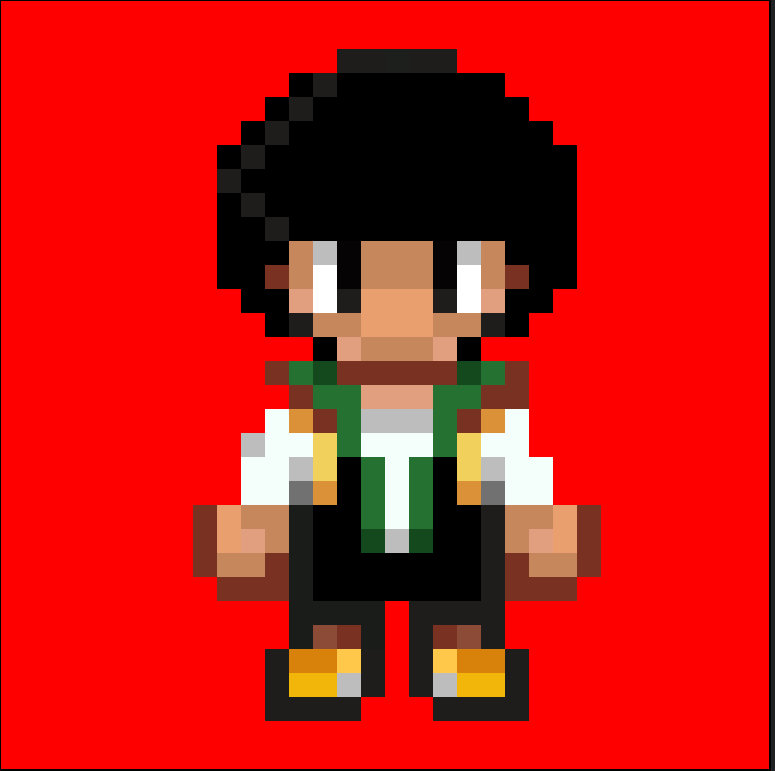
\includegraphics[width=0.5\linewidth]{figuras/player.png}
    \caption{Exemplo de retângulo associado a imagem do personagem principal, toda a area vermelha representa o retângulo associado ao \textit{player}}
    \label{fig:player}
\end{figure}

O método \textit{blit} do Pygame, é utilizado para desenhar imagens do tipo \textit{Surface} na tela. Essa função tem a seguinte assinatura.
\begin{itemize}
    \item \textit{\textbf{source}:} A imagem \textit{Surface} a ser desenhada sobre o \textit{Surface} atual;
    \item \textit{\textbf{dest (opcional):}} Posição onde será desenhado a imagem, sendo o padrão o canto superior esquerdo (0, 0);
    \item \textit{\textbf{area (opcional):}} A delimitação da área retangular para desenhar;
    \item \textit{\textbf{special\_flags (opcional):}} Controla como as cores do da imagem serão combinadas com a Superfície;
\end{itemize}

Na função \textit{draw\_menu} que é responsável por desenhar as informações na tela \textit{home} faz uso desse método, a imagem de \textit{background} é desenhada ao passar como parâmetro a imagem \textit{Surface} dessa interface. Para causar o efeito de iluminação sobre o index selecionado são usados também os parâmetros \textit{dest} e \textit{special\_flag}. O primeiro parâmetro é o ícone da imagem com o fundo branco, o segundo parâmetro é o retângulo com as coordenadas de onde está a seleção, este varia conforme o index, e o terceiro parâmetro é a \textit{special\_flag} \textit{BLEND\_RGB\_ADD }, essa \textit{flag} mistura os canais de cores RGB da imagem de \textit{background} com o ícone da imagem de fundo branco. A figura \ref{fig:blit-example} ilustra esse processo.

% a imagem de \textit{background} e os retângulos de seleção. Para causar o efeito de iluminação sobre os retângulos ao selecionar cada index é feito o uso do método \textit{blit} do pygame, esse método desenha uma imagem sobre outra imagem, sendo a primeira imagem o icone de exit com o fundo branco, e o destino onde será desenhado o retângulo com às coordenadas de cada botão, essa coordenada varia de acordo com o index. A fun tem a seguinte assinatura.
% % \begin{itemize}
% %     \item \textit{\textbf{source}:} A imagem \textit{Surface} a ser desenhada sobre o \textit{Surface} atual;
% %     \item \textit{\textbf{dest (opcional):}} Posição onde será desenhado a imagem, sendo o padrão o canto superior esquerdo (0, 0);
% %     \item \textit{\textbf{area (opcional):}} A delimitação da área retangular para desenhar;
% %     \item \textit{\textbf{special\_flags (opcional):}} Controla como as cores do da imagem serão combinadas com a Superfície;
% % \end{itemize}
% É graças ao quarto parâmetro \textit{special\_flags} que é possível causar esse efeito, usando a \textit{flag} \textit{BLEND\_RGB\_ADD } misturamos as cores RGB da mesma imagem com o fundo branco e é adicionado os canais de cor de origem aos canais de cor de destino.

\begin{figure}[h!]
    \centering
    
\includegraphics[width=1\linewidth]{figuras/blit_example.png}
    \caption{Exemplo de sobreposição de imagens com o método \textit{blit}}
    \label{fig:blit-example}
\end{figure}

A operação de \% (resto da divisão) é feita sobre o index para garantir que a opção selecionada pelo jogador seja somente uma das opções definidas. A variável \textit{new\_rect} contém o retângulo de coordenadas que será desenhado na tela. Todos os retângulos de seleção da tela inicial tem o tamanho fixo 123 x 90, o que muda é a posição que ele sera desenhado.

No Pygame um \textit{sprite} pode ser representado com a classe nativa \textit{Sprite}, herdar essa classe base e adicionar os atributos e métodos que são do nosso interesse é muito útil. Além disso o Pygame conta também com a classe \textit{Group}, nessa classe container é possível adicionar objetos do tipo \textit{Sprite}. A classe \textit{Group} pode ser utilizada para criar grupos de \textit{sprites} que o programador deseja que tenham comportamentos específicos. A classe suporta os seguintes operações padrão do Pygame.
\begin{itemize}
    \item \textbf{\textit{in:}}  testa se um Sprite está contido no grupo;
    \item \textbf{\textit{len:}}  retorna o número de Sprites contidos no grupo;
    \item \textbf{\textit{bool:}}  verifica se algum Sprite está contido no grupo;
    \item \textbf{\textit{iter:}}  itera todos os Sprite no grupo;
\end{itemize}

% especialmente se usada em conjunto com a classe container \textit{Groups}. Nessa classe é possível adicionar Sprites que podem ser criados para comportamentos específicos, por exemplo, se queremos criar um grupo de sprites que tenham o comportamento de matar o jogador em caso de colisão, poderíamos criar um \textit{Group} chamado \textit{''hitkill\_sprites''} e nele adicionar todos os sprites que queremos que tenha esse comportamento. Para realizar a ação de matar o \textit{player} bastaria percorrer \textit{hitkill\_sprites} e verificar a colisão, 

% veja no exemplo da listagem \ref{lst:hitkill-sprite}
% \lstinputlisting[label=lst:hitkill-sprite, caption=\textit{Hitkill Sprites}, language=Python, float=htpb]{codigos/hitkill_sprites.py}
\lstinputlisting[label=lst:game, caption=Classe \textit{Game}, language=Python, float=htpb]{codigos/game.py}

No jogo existem cinco tipos de \textit{Groups} podendo um \textit{sprite} pertencer a mais de um grupo simultaneamente, a (listagem \ref{lst:game}) mostra a classe \textit{Game} onde é feito o uso recurso:
\begin{itemize}
    \item \textit{\textbf{collision\_sprites: }}Grupo que contém todos os \textit{sprites} colidíveis do jogo no mapa atual;
    \item \textit{\textbf{character\_sprites: }}Grupo que contém todos os \textit{sprites} de personagens do game no mapa atual;
    \item \textit{\textbf{transition\_sprites: }}Grupo que contém todos os \textit{sprites} de colisão no mapa atual;
    \item \textit{\textbf{dialogs\_sprites: }}Grupo que contém todos \textit{sprites} que geram uma caixa de diálogo no mapa atual;
    \item \textit{\textbf{interaction\_sprites: }}Grupo que contém todos os \textit{sprites} do jogo que são interativos;
\end{itemize}

A classe \textit{Game} também responsável por inicializar todas as variáveis, áudios, e \textit{assets} que são pertinentes ao jogo. É nessa classe que são chamadas as função \textit{import\_assets} e \textit{setup}, sendo a primeira para carregar todos os \textit{assets} do jogo para o programa, e a segunda para fazer a inicialização do mapa inicial. 

% inicial do jogador essa será explicada na listagem \ref{lst-import-assets} e chama também o método \textit{setup} listagem \ref{lst-setup} que que carrega e inicializa o mapa inicial.


\lstinputlisting[label=lst-import-assets, caption=Import Assets, language=Python, float=htpb]{codigos/import_assets.py}
\clearpage
O método \textit{import\_assets} (listagem \ref{lst-import-assets}) é responsável por fazer a importação e alocação de todos os mapas e assets do jogo. A atribuição desses \textit{assets} é feita através de um dicionário para melhor organização do código. Abaixo na tabela \ref{tbl-especificacao-dicionario} da especifica mais as possíveis chaves e valores.


\begin{table}[h!]
	\caption{Especificação dos dicionários de assets.}
	\label{tbl-especificacao-dicionario}
	\centering
	\renewcommand{\arraystretch}{2}
	\begin{small}
		\begin{tabular}{ | p{35mm} | p{35mm} | p{65mm} |}\hline \rowcolor{MidnightBlue}
                \hline
                Variável & Chave & Valor \\
                \hline
                \textit{tmx\_maps} & \textit{map\_name} & Arquivo TMX \\ 
                \hline
                \multirow{3}{4em}{overworld\_frames} 
                & \textit{characters} & \textit{Sprites} de personagems \\ 
                & \textit{water} & \textit{Sprites} de água \\ 
                & \textit{lake} & \textit{Sprites} das bordas do lago \\ 
                \hline
                \multirow{3}{4em}{fonts} 
                & \textit{dialog} & Fonte do diálogo \\ 
                & \textit{bold} & Fonte negrito \\ 
                & \textit{regular} & Fonte do inventário e computador \\ 
                & \textit{regular\_mid} & Fonte igual a anterior com tamanho 22 \\ 
                & \textit{regular\_big} & Fonte igual a anterior com tamanho 34 \\ 
                \hline
                \multirow{3}{4em}{interface\_frames} 
                & \textit{interface} & \textit{Sprites} com os \textit{layouts} da interface \\ 
                & \textit{items} & \textit{Sprites} com os items do inventario \\ 
                & \textit{interactive\_objects} & \textit{Sprites} que tem algum tipo de animação ao interagir \\ 
                \hline

                \end{tabular}
	\end{small}
\end{table}

\clearpage
\lstinputlisting[label=lst-setup, caption=Setup, language=Python, float=htpb]{codigos/setup.py}
\clearpage
O método a anterior \textit{setup} (listagem \ref{lst-setup}) tem a função de carregar o mapa passado como parâmetro e iniciar todos os \textit{sprites} presentes no mapa passado como argumento. Essa função é chamada ao iniciar um novo jogo, e também caso o jogador mude para outro mapa do \textit{game}. Como pode conter um mapa na memória quando essa função for chamada, o primeiro passo é limpar os \textit{sprites} do mapa anterior. Após isso é feito uma série de interações sobre todas as camadas presentes no mapa \textit{.tmx} que foram criadas no editor de mapas. É nessa etapa que é realizada a atribuição de cada \textit{sprite} com os seus respectivos grupos, sendo eles.
\begin{table}[h!]
	\caption{Tabela especificando os tipos de \textit{sprites} presentes em Super Labes World}
	\label{tbl-especificacao-sprites}
	\centering
	\renewcommand{\arraystretch}{3}
	\begin{small}
		\begin{tabular}{ | p{37mm} | p{23mm}  | p{52mm} | p{30mm} | }\hline \rowcolor{MidnightBlue}
			\centering{\textbf{Classe}} & \centering{\textbf{Camadas}} & \textbf{Descrição} & \textbf{Grupos} \\\hline		
                \centering{\textit{Sprite}} & \centering{\textit{Terrain, Terrain Top, Terrain Objects}} & {Classe com os tiles da camada mais baixa sem colisões} & {\textit{all\_sprites}} \\\hline
                \centering{\textit{AnimatedSprite}} & \centering{\textit{Lake, Lake Edges}} & {Classe com tiles animados do lago sem colisão} & {\textit{all\_sprites}} \\\hline			
                \centering{\textit{CollidableSprite}} & \centering{\textit{Objects}} & {Classe com os sprites de objetos do jogo com colisão} & {\textit{all\_sprites, collision\_sprites}} \\\hline		
                \centering{\textit{InteractiveSprite}} & \centering{\textit{Interactive Objects}} & {Classe com os sprites com interação com colisão} & {\textit{all\_sprites, collision\_sprites, interactive\_sprites}} \\\hline	
                \centering{\textit{CollisionSprite}} & \centering{\textit{Collisions}} & {Classe com as colisões sem uma imagem} & {\textit{collision\_sprites}} \\\hline		
                \centering{\textit{CollidableDialogSprite}} & \centering{\textit{Dialogs}} & {Classe com os sprites de diálogo} & {\textit{dialog\_sprites}} \\\hline		
                \centering{\textit{TransitionSprite}} & \centering{\textit{Transitions}} & {Classe que armazena os sprites de transição sem imagem} & {\textit{transition\_sprites}} \\\hline		
                \centering{\textit{Player}} & \centering{\textit{Entities}} & {Classe do jogador principal} & {\textit{all\_sprites}} \\\hline			
		\end{tabular}
	\end{small}
\end{table}
\begin{table}[h!]
	\caption{Tabela especificando os tipos de \textit{sprites} presentes em Super Labes World}
	\label{tbl-especificacao-sprites}
	\centering
	\renewcommand{\arraystretch}{3}
	\begin{small}
		\begin{tabular}{ | p{37mm} | p{23mm}  | p{52mm} | p{30mm} | }\hline \rowcolor{MidnightBlue}
			\centering{\textbf{Classe}} & \centering{\textbf{Camadas}} & \textbf{Descrição} & \textbf{Grupos} \\\hline	
                \centering{\textit{Character}} & \centering{\textit{Entities}} & {Classe para representar as entidades de personagens do jogo} & {\textit{all\_sprites, collision\_sprites, characters\_sprites}} \\\hline	
		\end{tabular}
	\end{small}
\end{table}

\clearpage
Ao jogador entrar em uma batalha o programa bloqueia a entrada de comandos do \textit{game loop} principal e muda para o contexto da classe \textit{Battle}. A função que contém esse loop da função \textit{update} é mostrada a seguir na listagem \ref{lst-update-battle}.
\lstinputlisting[label=lst-update-battle, caption=Loop da classe \textit{Battle}, language=Python, float=htpb]{codigos/update_battle.py}
\begin{enumerate}
    \item \textit{\textbf{battle\_timer.update:}} Função que atualiza a contagem de tempo na batalha;
    \item \textbf{\textit{check\_end\_battle:}} Função que verifica se o fim da batalha chegou, ou seja todas as questões foram respondidas, ou o jogador errou 30\% do total de perguntas e chama a função de \textit{callback} para o \textit{loop} principal com uma lista de inteiros, sendo 0 para respostas erradas, 1 para respostas corretas;
    \item \textbf{\textit{input: }} Função que captura a entrada de comandos do jogador e lida com os índices, similar ao menu inicial explicado em \ref{lst-home};
    \item \textbf{\textit{display\_surface.blit:}} Função que desenha o background da batalha;
    \item \textbf{\textit{draw\_rectangles:}} Função que desenha os retângulos associados as opções de escolha do jogador, similarmente como já explicado em \ref{fig:blit-example}
    \item \textbf{\textit{draw\_questions:}} Função que desenha na tela o texto da questão atual
    \item \textbf{\textit{draw\_answers:}} Função que desenha o conteúdo da resposta de acordo com a opção que o jogador está;
    \item \textbf{\textit{draw\_character\_info:}} Função que desenha as informações do professor na tela (nome e level);
    \item \textbf{\textit{draw\_characters:}} Função que realiza o desenho e a animação dos dos personagens nessa tela será mais detalhada a seguir;
    \item \textbf{\textit{draw\_dialog:}} Função que desenha o diálogo do professor ao responder a questão;
\end{enumerate}

A função abaixo \ref{lst-check-answer} é chamada ao jogador apertar barra de espaço sobre alguma das opções da batalha, ela seta a variável \textit{error\_mode} e escolhe um texto randomicamente de acordo com a resposta da questão. Essas que são usadas para as funções de desenhar o texto na tela e também para a animação do personagem.
\lstinputlisting[label=lst-check-answer, caption=Função chamada ao jogador escolher uma opção na batalha, language=Python, float=htpb]{codigos/check_answer.py}


\clearpage
\section{Personagens}
\label{sec:personagens}
Os personagens de um jogo são uma peça fundamental especialmente para um jogo do gênero RPG, eles desempenham um papel central na construção da experiência narrativa e interativa e enriquecem fortemente a ambientação do jogo, esse capítulo vai abordar em mais detalhes como foi feita a criação de personagens

Os \textit{sprites} dos personagens do jogo foram desenhados no software Aseprite discutido na seção \ref{sec:aseprite} e exportados para o formato PNG (Portable Network Graphics). Cada \textit{sprite} de personagem tem o tamanho (512 x 512), mas no programa essa imagem é subdividida em 16 quadrados de tamanhos iguais (128 x 128) como mostra a figura \ref{fig:player-animation}

A adição de personagens ao jogo é feita pela ferramenta Tiled citado na seção \ref{sec:tiled}. No software existe um recurso chamado \textit{Insert Point}, os pontos são os objetos mais simples possíveis de adicionar a um mapa, eles representam apenas uma localização e não podem ser redimensionados ou girados, mas é possível atribui-los com metadados. Esses metadados podem ser utilizados no Pygame para a identificação de cada personagem. Em nosso caso os metadados inseridos foram, e pode ser vista pelas figuras \ref{fig:tiled-house} e \ref{fig:tiled-player-properties}.
\begin{itemize}
    \item \textbf{\textit{character\_id: }} Identificador do personagem. Todas as características do personagem (diálogos, \textit{frames}, questões, etc) são dependentes desse \textit{id} ;
    \item \textbf{\textit{direction: }}Define qual é a direção inicial do jogador;
    \item \textbf{\textit{pos: }} Contém o mapa anterior que o \textit{player} estava antes da transição. Isso é necessário porque todo mapa contém pelo menos duas possíveis transições (ida e volta). Essa variável então é usada para diferenciar cada posição do jogador e o programa conseguir desenhar o jogador na posição correta. (Propriedade é relativa somente ao player);
\end{itemize}

\begin{figure}[h!]
    \centering
    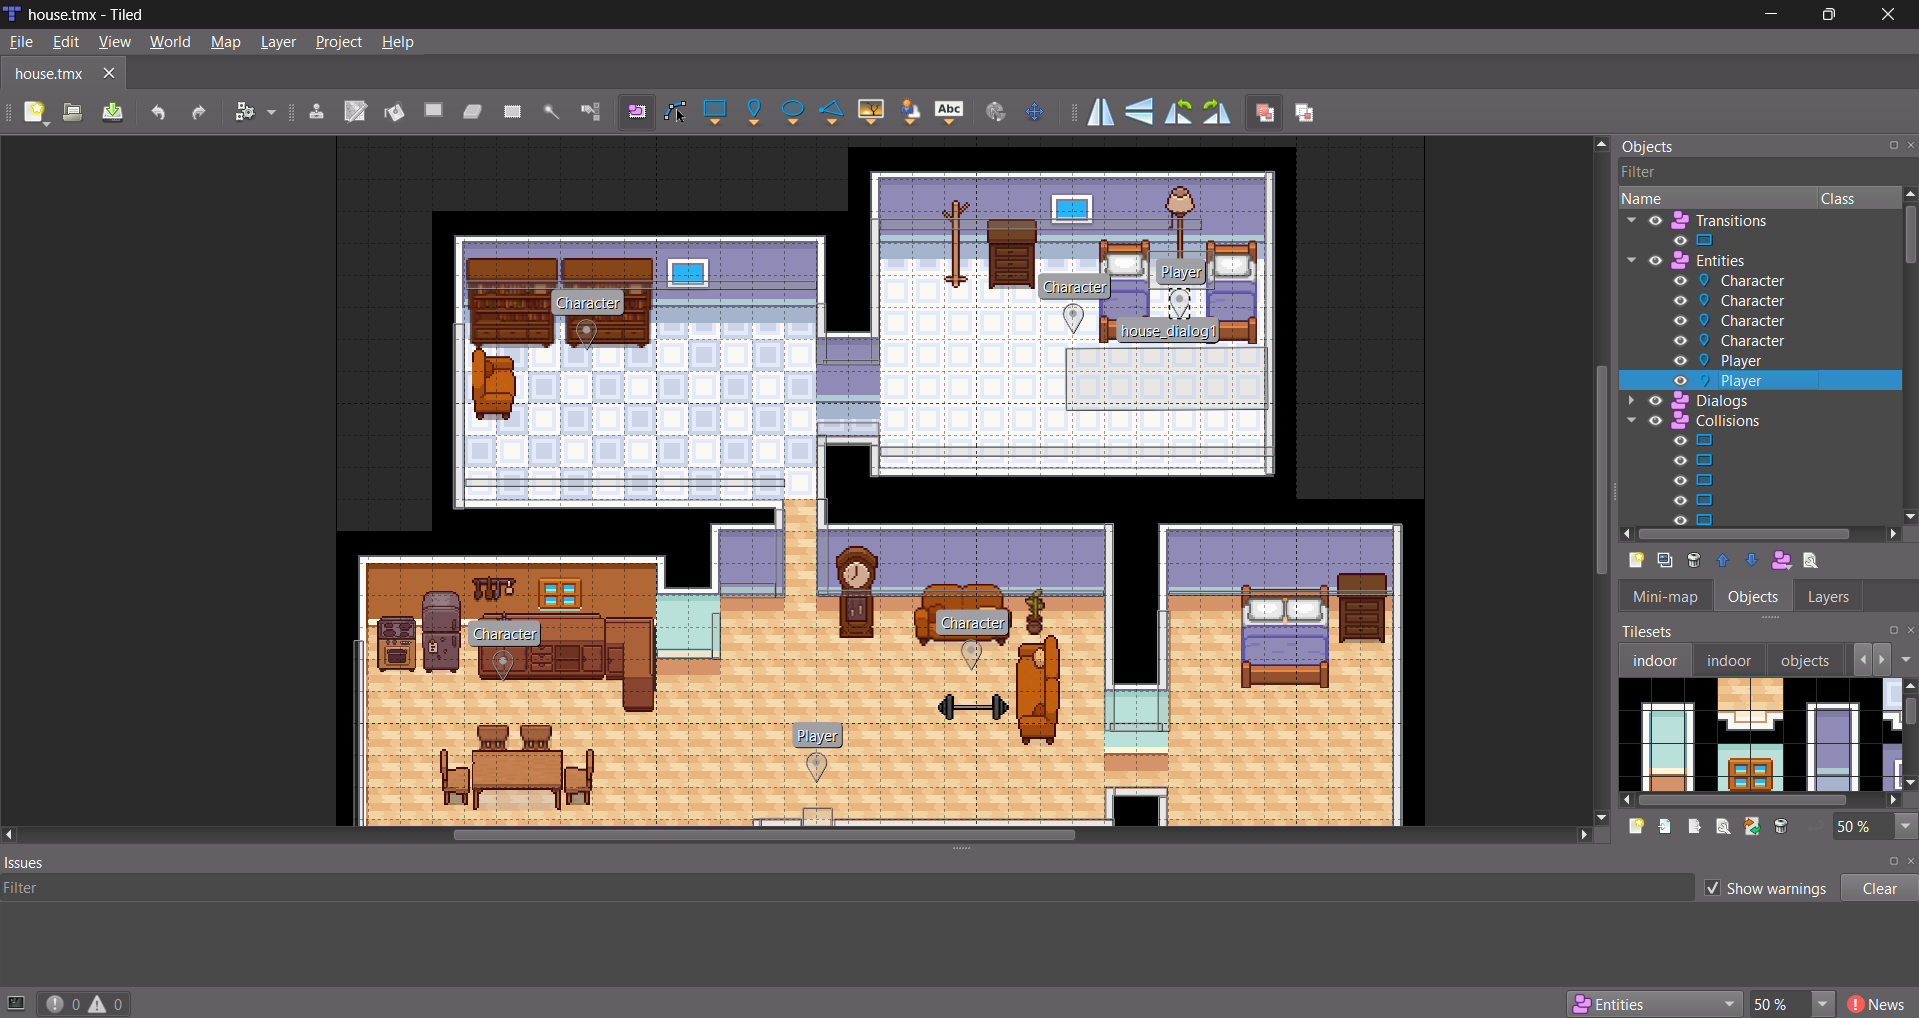
\includegraphics[width=1\linewidth]{figuras/tiled-house.png}
    \caption{Posicionamento de Objetos no Software Tiled }
    \label{fig:tiled-house}
\end{figure}

\begin{figure}[h!]
    \centering
    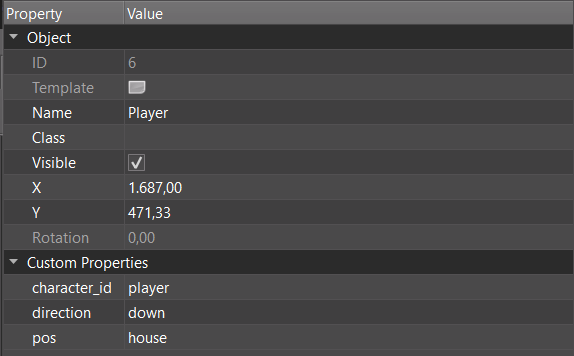
\includegraphics[width=1\linewidth]{figuras/tiled-player-properties.png}
    \caption{Propriedades da Entidade Player no Tiled}
    \label{fig:tiled-player-properties}
\end{figure}

\clearpage
Animação como explicado na seção \ref{sec:animacao} é uma ilusão gerada pela sequência de imagens sendo alternadas a uma determinada velocidade. No Super Labes World para fazer uso dessa técnica é criado um dicionário, sendo a chave o nome do estado em que o jogador se encontra e o valor um vetor de imagens relacionadas aos possíveis estados. A figura mostra a figura a seguir:
\begin{figure}[h!]
    \centering
    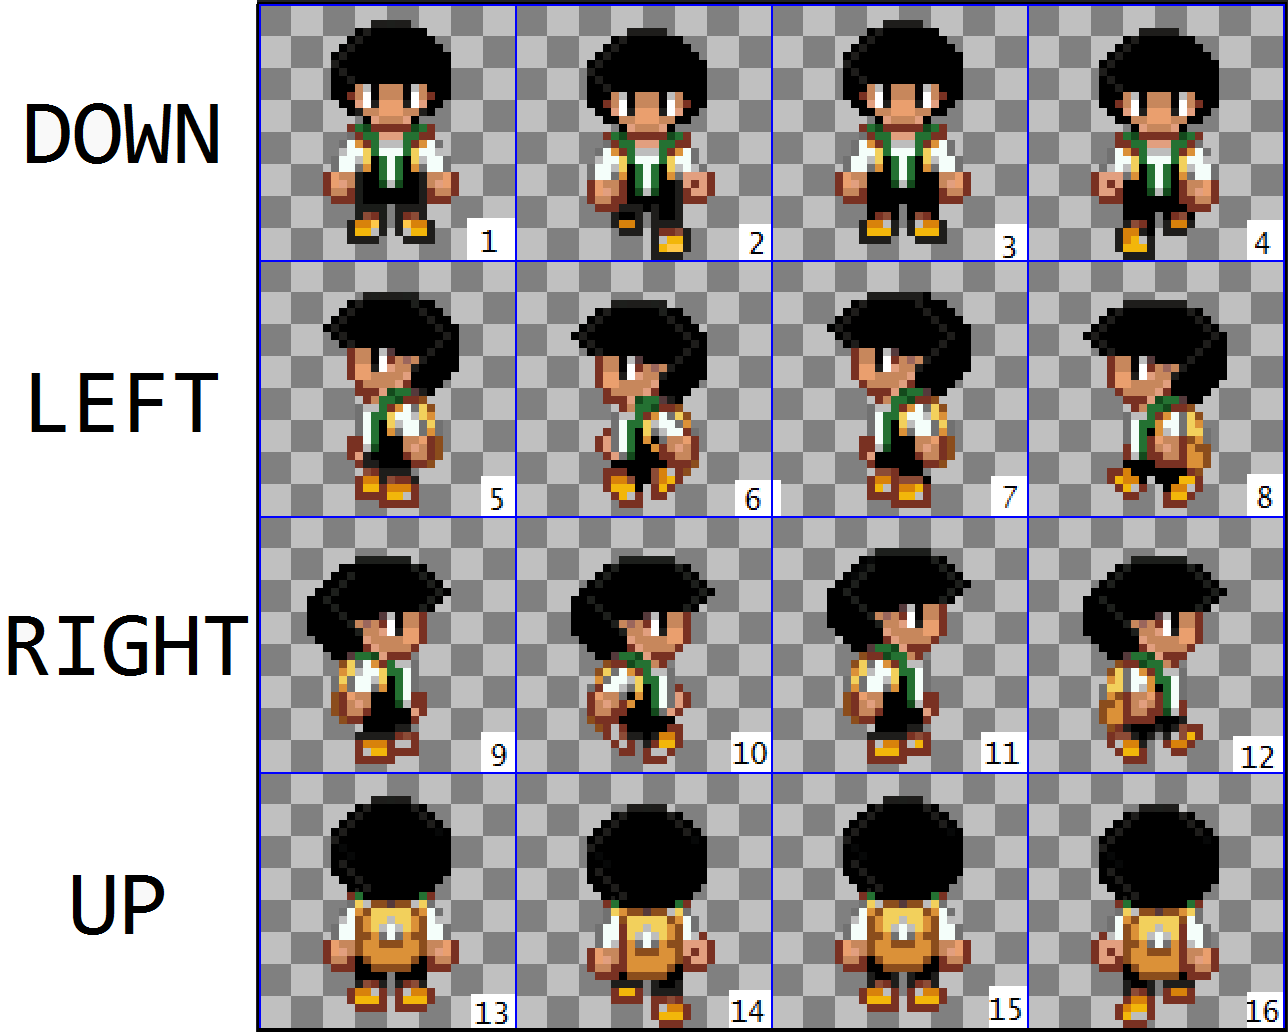
\includegraphics[width=1\linewidth]{figuras/player-animation.png}
    \caption{\textit{Sprite} de Animação dos \textit{Player} }
    \label{fig:player-animation}
\end{figure}

Cada chave do dicionário contém quatro imagens (frames), também são criados quatro estados adicionais com o sufixo \textit{''idle''} (parado) correspondente a cada direção. Isso é feito para que quando o jogador pare a movimentação, o programa mude o \textit{frame} para a direção atual do player porém parado. 
\begin{enumerate}
    \item \textit{\textbf{down:}} Mantém as imagens 1, 2, 3 e 4;
    \item \textit{\textbf{down\_idle:}} Mantém a imagem 1;
    \item \textit{\textbf{left:}} Mantém as imagens 5, 6, 7 e 8;
    \item \textit{\textbf{left\_idle:}} Mantém a imagem 5;
    \item \textit{\textbf{right:} Mantém as imagens 9, 10, 11 e 12};
    \item \textit{\textbf{right\_idle:}} Mantém a imagem 9;
    \item \textit{\textbf{up:}} Mantém as imagens 13, 14, 15 e 16 ;
    \item \textit{\textbf{up\_idle:}} Mantém a imagem 13;
\end{enumerate}

% detalhar mais aqui
Para realizar a animação do personagem principal no código foram criados os seguintes métodos.
\lstinputlisting[label=lst-player-animation, caption=Player animation, language=Python, float=htpb]{codigos/player_animation.py}
\begin{itemize}
    \item \textit{\textbf{animate:}} Intercala os frames do personagem de acordo com o retorno da função \textit{get\_state:} enquanto estiver sendo chamada;
    \item \textit{\textbf{get\_state:}} Retorna a direção atual do jogador;
    \item \textit{\textbf{input:}}  Retorna um vetor [x, y] direcional normalizado relativo as teclas que o jogador jogador pressionou;
    \item \textit{\textbf{move:}} Realiza a movimentação do personagem de acordo com o vetor obtido anteriormente;
    \item \textit{\textbf{update:}} Função que é chamada no \textit{loop} principal do jogo, é a partir dela que todas as anteriores são chamadas;

\end{itemize}
% Uma função que fique intercalando os frames de acordo com o estado atual do jogador, uma função que retorne o estado atual do jogador, uma função para capturar a entrada de teclado do jogador e retorne um vetor com a direção, uma função para movimentação e uma função para atualização. Essas funções são descritas a seguir na listagem \ref{lst-player-animation}.

% A função \textit{animate} alterna a imagem do personagem a partir da variável \textit{frame\_index} essa cujo valor vai aumentando conforme o \textit{delta time} e \textit{ANIMATION\_SPEED} que é uma constante usada para definir quão rápido serão as animações do jogo. A função \textit{get\_state} retorna qual estado que o jogador está, que é a chave para o dicionário de frames. A função input a função \textit{move} realiza a movimentação do personagem propriamente dito, e a update é o event loop relativo ao player


Ao carregar o sprite do personagem para o jogo percebe-se que a area relativa ao retangulo é consideravelmente menor do que a área desenhada \ref{fig:player}.
% existe um problema, o retângulo do player é muito maior do que a imagem do personagem,
No Pygame existe um método do Pygame para lidar com isso, o método \textit{inflate}. Essa função diminui o tamanho de um retângulo caso seja passado um valor negativo de parâmetro, e aumenta caso o valor seja positivo. É feito isso e atribuímos a variável \textit{hitbox} essa variável do tipo \textit{Rect} representa a área colidível do jogador. A listagem \ref{lst-player-hitbox} mostra a utilização do método e a figura \ref{fig:player-hitbox} simula o resultado diminuindo a largura pela metade e 60 píxels de altura.

\begin{lstlisting}[language=Python,breaklines, caption= Uso da Função \textit{inflate}, label= lst-player-hitbox]
self.hitbox = self.rect.inflate(-self.rect.width / 2, -60)
\end{lstlisting}
\begin{figure}[h!]
    \centering
    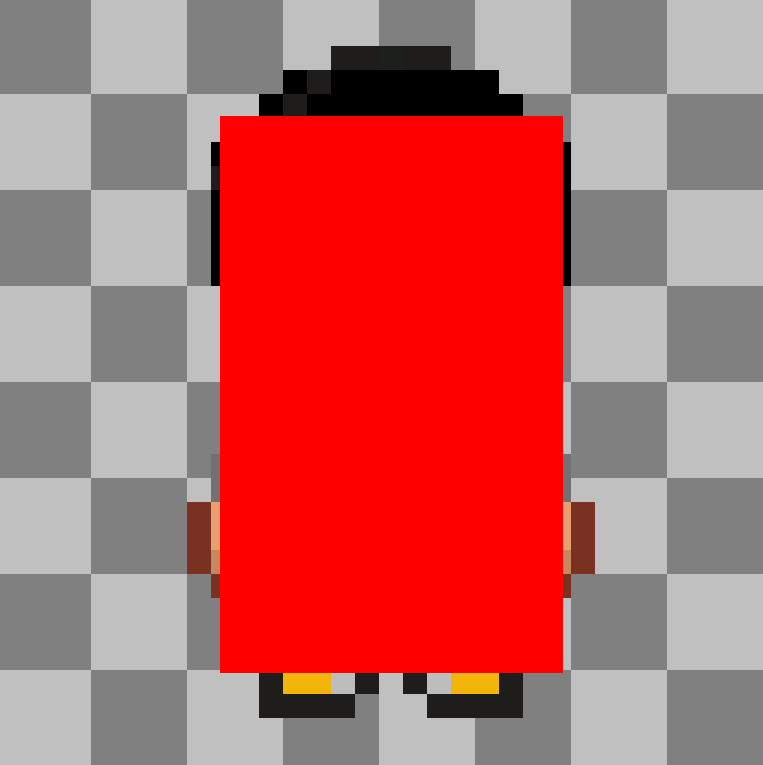
\includegraphics[width=0.7\linewidth]{figuras/player-hitbox.png}
    \caption{\textit{Hitbox} do personagem principal após o a chamada do método \textit{blit}}
    \label{fig:player-hitbox}
\end{figure}

\clearpage
Na batalha, os personagens são animados pela função \textit{draw\_characters}. A animação só ocorre após a primeira resposta, e depende da variável \textit{error\_mode}, obtida logo após uma resposta do jogador. caso o valor seja verdadeiro, significa que o jogador errou, a movimentação do \textit{sprite} é vertical (eixo y), os frames utilizados será o dicionário com a chave ''\textit{up}'' \ref{fig:player-animation}. Caso contrário a movimentação é lateral (eixo x) e os frames utilizados serão os com a chave ''\textit{left}'' do dicionário.
\lstinputlisting[label=lst-update-battle, caption=Função responsável por desenhar as animações da classe \textit{Battle}, language=Python, float=htpb]{codigos/draw_characters.py}

